\chapter{Testing and User Feedback}
\label{chap:testing}

\section{Unit testing}

\begin{figure}[h!] 
    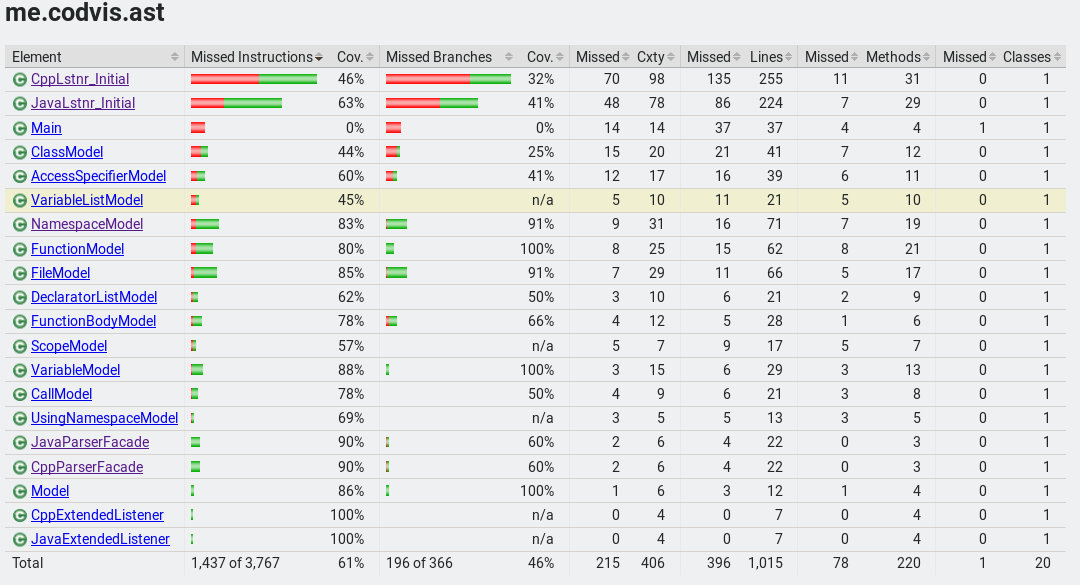
\includegraphics[width=\textwidth]{inc/images/test/JavaTests.png}
    \caption{Test summary of different Java \gls{antlr}  parser files.}
    \label{fig:testJava}
\end{figure}


Unit testing was done in Java \gls{antlr} parser using JUnit. In Java \gls{antlr} parser unit tests were written for most of the models and listeners. 
The goal of unit testing was to test as many as possible instructions. Trivial functionalities such as getters and setters were not tested.
Each model is tested to see if only data of compatible types would be inserted and would return the correct data once asked for \gls{json}. Listeners were tested to see if they were able to parse specified context and were able to create correct models that could return correct data within \gls{json}. Testing in Java was not complete due to prioritization of other important tasks. 

\begin{figure}[H] 
    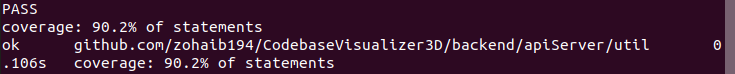
\includegraphics[width=\textwidth]{inc/images/test/apiServer_testCoverage_util.png}
    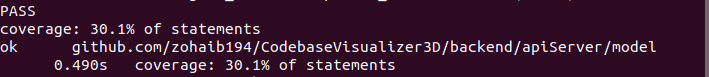
\includegraphics[width=\textwidth]{inc/images/test/apiServer_testCoverage_model.png}
    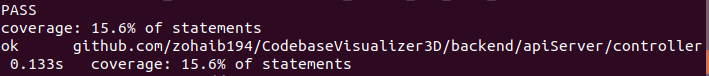
\includegraphics[width=\textwidth]{inc/images/test/apiServer_testCoverage_controller.png}
    \caption{Test summary of different Go \gls{api} files.}
    \label{fig:testGO}
\end{figure}


In Go \gls{api} the goal was to test the \gls{api} entry points through \gls{frontend} using a \gls{js} testing framework called \gls{ava}, but functionality used for entry point within Go should be test using Go test. As shown in figure \ref{fig:testGO}, util package is a custom package for different logging functionalities that are used through out the Go \gls{api} and almost all functionalities are unit tested. In model package only the database functionalities are tested. In controller package one of the REST endpoint was tested. This happened before the goal of testing in Go \gls{api} was set. The endpoint accounts for multiple good and bad tests cases. To create a general structure in testing code for Go a sublime package was used called gotests \cite{github:gotestsplugin}.

\begin{figure}[H]
\noindent\rule{\textwidth}{1pt}
\begin{lstlisting}[language=JavaScript, caption= {JSON structure for a valid test case}, label={lst:testCase}]
{
	name: "Valid - new repo - sendAddRequest",
	websocketURL: "ws://localhost:8080/repo/add",
	payload: {
		uri: "https://github.com/example/ECS.git"
	},
	wantMessage: {
		length: 1,
		messages:
		[
			{
				statuscode: 202,
				statustext: "Accepted",
				body : {
					status: "Cloning"
				}
			}
		]
	},
	wantCloser: {
		reason: {
			statuscode: 201,
			statustext: "Created",
			body: {
				status: "Done"
			}
		}
	}
}
\end{lstlisting}
\noindent\rule{\textwidth}{1pt}
\end{figure}

In \gls{frontend} only one of the end points were able to be tested due to time prioritization. The endpoint is implemented as \gls{websocket} and as shown in the listing \ref{lst:testCase}, \gls{json} structure was used as for a test case. This test would add a new repository link and expects onMessage and onClose channel of \gls{websocket} to receive data as shown.

\section{Code Quality}
The team put a lot of effort looking into professionalism and best practises when it comes to code. To maintain high code quality there were a number of steps taken:

\begin{itemize}
    % Merge request issues
    \item Merge requests in Github was used so any members code would be looked through by at least one member and errors would be reported and not merged until resolved. This was also very helpful in the sense of giving all members a peek into progress and what was done in the areas not touched by them. 
    % Documentation
    \item Documentation were prioritized throughout the project both commenting for auto-generated documentation but also self-documenting code.
    % Convensions and Best practises
    \item Conventions and Best practises were also prioritized. They are always good to follow because they are tried and tested informal rules to produce easily maintainable and high quality code \cite{wiki:bestCodingPractises}. 
    % Dependency quality assurance
    \item Dependencies, inspiration and ideas were taken form what the team considered professional grade projects, libraries or frameworks. If they are still active in development or maintenance, any recent updates, number of people who contributed, general good structure and open-source were all items we would check for on any project to determine whether it was created in a professional setting. For example if a project has one contributor or significantly lacking in number of commits for the apparent level of complexity, it would not be considered as a professional grade project unless the code itself is regarded as being good. % Kent: Contradictory? Too much repetition? Too segmented?
\end{itemize}

\section{User studies}
User studies are very important in the sense that it's a controlled trial of the application. The developers can get an insight into how the users will use the application and give feedback on improvements. This usually results in a higher quality product and the developers can ensure that the application is easy-to-use and stable \cite{kosara2003user, sridhar1995understandingTheUser}. As this project is more of a research based project, much of the application is more of a prototype and might not be intuitive. The group therefore performed a user study that is available in Appendix \ref{app:userStudies} to get some ideas on how to improve the system. 

\subsection{User categorization}
The users of this application are categorized in to three types, Student, Lecturer and Professional: 
\begin{itemize}
    \item Student is anyone looking up a library for any number of reasons. 
    \item Lecturer is anyone trying to teach something about a concept and uses this application for this purpose. 
    \item Professional is anyone using the application in any professional or corporate setting.
\end{itemize}

The intended result from this classification is that the different groups will have different ways of viewing the application. Students might have a more simplistic view and initial understanding of the system and might therefore focus more on usability and basic functionalities. Lecturers might be more analytical and will focus a little more on what the system will give them, how it gives this information and why its represented the way it is. The professionals might view the application from a industrial perspective and might give feedback about \gls{it} related industrial standards, quality and more advanced features.

\subsection{Testing methodology}
\newacronym{gdpr}{GDPR}{General Data Protection Regulation}
Before the participant answer the questions in the questionnaire, they're instructed to look at a predetermined code-example and asked to draw their visualization that represents the given code-example, as well as some basic tasks that will probe how they use the application. Information like where they look to improve efficiency of retrieving information, mouse movements to see indications on though process and any control inputs to look for navigability issues and intuitiveness within the visualization.

The primary reasons for selecting these questions is that some will give insights into how the application is used and how easy it is to retrieve any additional information from the home page. Others will probe the visualization it self and give an insight to whether it's intuitive and easy to navigate. Some questions will probe the GUI within the visualization and it's layout for retrieving/viewing any information and others will give a general understanding of their role but will not be sufficient to identify the individual.

In a in-formal user study it's important that one doesn't break any \gls{gdpr} laws which means no recording of any data that can identify the person testing the application without users consent, the ability for the user to request or delete their data and that is deleted within reasonable time. \cite{lovdata:gdpr}. 

\section{Results}
As the user study only involved nine participants, the data is not extensive enough to make any definitive conclusions, the group is however confident that data gathered could still be used to guide future work. 

\subsection{Navigation and UI}
The questionnaire indicated that the users felt the navigation was mostly intuitive, but wanted information on how it worked rather than leaving it to guesswork. The activities however, indicated that many of them struggled and did not see it as intuitive, especially moving into the data-structures and sideways movement. One thing that seemed clear was that initial camera position, before moving, was too close. This made it difficult for the user to orient themselves. It was also mentioned by a user that information about current orientation would be beneficial.

Several users tried to use the static windows for navigation. This was a feature the team had previously thought about, but had not implemented due to time constraints. It became clear that this should have been prioritized higher.

\subsection{Visualization and interaction}
Most users indicated that the choice of colors and shapes were good, and had little problem identifying the relationship between the visualization and code. 

Several users had problems with finding the implementation, whether this had to do with unclear terminology or if changes made by the interaction was hard to spot is unclear. Most users clicked the function to get the implementation as expected, but some did not notice the update in the separate window or noticed but did not draw the connection. An improvement might be to add syntax highlighting, increase the size of the window or highlight to active function in the visualization.

\subsection{Proposed features}
\begin{itemize}
    \item Information about how to navigate
    \item Information about orientation
    \item Customized navigation option
    \item Save and restore camera position
    \item Ability to change visuals
    \item Sidebar navigation
    \item Position reset button
    \item Toggle visibility
    \item Information about call order
    \item Integrate source code into visualization
\end{itemize}

Most of the suggestions had been discussed earlier and was planned if time allowed for it, but there seem to be a higher want for enhanced navigation features than expected. 